\subsection{The challenges of thread switching}
\label{chap:Threading}
That challenges of thread switching in ARM stem from the difficulty in storing a threads' context in a way which is recoverable from any point without losing any state. A good place to tackle this problem is to start from looking at how a procedure call works in ARM. Procedure calls in arm are somewhat similar in concept, but they differ in scope. The procedure calls \cite{arm_man} I used in ARM consisted of the following steps
\begin{itemize}
	\item Move the LR onto the stack 
	\item Push non-parameter registers
	\item Execute the required procedure
	\item Update the defined output registers
	\item Recover the non-parameter registers from the stack
	\item Pop the LR back
	\item Return to the call location
\end{itemize} % Might be good to compare my procedure calls to the arm standard
This structure for a procedure call allows me to nest procedure calls within each-other where necessary. Where the thread switching protocols differ is that they can't merely push registers to the stack. This is because, for each thread running, neither thread should have to concerned with the others' existence. Each thread should be able to access the resources available without any concern that the other threads could be modifying the contents of the stack or a threads registers. In a sense threads should be invisible to each other. This raises several issues:
\begin{itemize}
	\item When should I run the context saving procedure to perform the time slicing?
	\item Which modes can you actually interrupt, and which modes need to be handled atomically?
	\item How do you keep the user's stack consistent for each thread?
	\item How do you store and load a threads' context without corrupting the registers or CPSR?
\end{itemize}
\subsubsection{When is the time-slicing procedure called?}
This is the easiest of the challenges above to solve. One of the plug-ins provided in the installation for Komodo is a configurable timer which can cause an interrupt. This is a natural entry point for the time slicing procedure, as a successfully implemented interrupt should be handled invisibly relative to the currently executing program. This is essentially what I want to occur. The executing program halts for the interrupt, which then gives control to another program, until another time slice is complete and control is returned to the original program. Of course in this example I am using two threads, but it can generalise to more threads. 
\subsubsection{When can I safely interrupt?}
This is the next easiest challenge to solve. While it is possible to implement complex behaviours in ARM such as nested interrupts without extra hardware support, the software complexities required to implement it are usually not worth the benefits. Allowing nested interrupts can make it very convoluted (but not impossible) to return the processor state to its precise state before any interrupts had occurred. The only upside of this added complexity that I can see is that you can reduce the latency in which you handle interrupts, which I could see being useful in some situations (such as a real-time system) but not in this one. Therefore, the solution as I see it is to leave interrupts as disabled during a standard interrupt call. Similarly, I would disable interrupts during a supervisor call, as it would complicate saving the state of the processor as I would need to ensure that the supervisor stack was kept consistent. Again, this is possible to do, but it does not yield many benefits for me.
\subsubsection{How do I ensure the user stacks consistency?}
The solution to this problem looks more simple than it is to implement. I chose to assign each thread its own user stack to ensure that each program can operate on its own stack independently. The memory space assigned to each thread is statically assigned on start up according to a constant MAX\_THREADS. This constant defines the maximum number of threads which I allow, and allocates memory accordingly and divides it between the threads.  Once I have created this memory space, when I give a call to create a new thread, I can pick the first free stack space and calculate a stack pointer for it. The reset procedure also has to account for this set-up as the main thread has to be treated in same way as any other thread.  This means that on reset, the correct data must be inserted into my process control block (PCB) to mimic a call to my thread creation procedure. Now that each thread has its own stack pointer, saving my stack during a context switch is as simple as saving my stack pointer.
\newpage
\subsubsection{How do you store and load a threads' context?}


\begin{wrapfigure}{l}{0.5\textwidth}\centering
	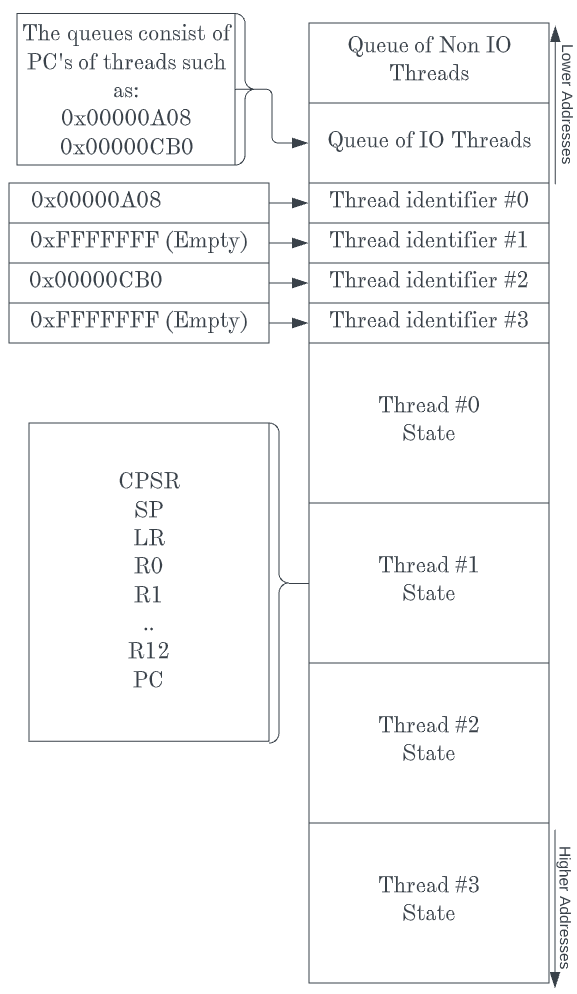
\includegraphics[scale=0.335]{figures/PCB.png}
	\caption{The memory layout of the PCB.}
	\label{fig:PCB}
\end{wrapfigure} 
This is the hardest problem I encountered when implementing threading. The loading and storing of a threads' context requires me have an organised way of storing and recovering each context. This is when the PCB comes in. The PCB consists of the setup as seen in  Figure \ref{fig:PCB}. The PCB represent the state of saved threads at any given point. A threads state is represented by first storing its PC in either the IO thread queue or the Non IO thread queue, depending on whether it was created with access to the virtual keyboard.
Once a thread is pushed onto a queue, its PC is used as an identifier in the thread identifier block. This block is an unsorted block, in which a thread is inserted at the first free location as designated by a -1 (0xFFFFFFFF). The index of the threads PC then acts as an index for the thread states. The thread state at that index will then hold the actual registers for the thread. The registers are stored in the order shown on the left with the CPSR, SP and LR being stored before R0 - R12 and then the PC. An option I had to consider when creating this memory structure was how I was going to identify my threads. Most modern computers use a unique process identifier (PID) to reference a thread or process. %Probably a good point for a reference about operating systems
I briefly considered implementing this rather than identifying threads via their program counter however I felt that PIDs are more useful for a processor where a process might be executed on an arbitrary core rather than a single core. In my system, as there is only one 'core' nothing can change the PC without running the code, so it acts as a decent primary key.

The order of the registers is very specific in order to aid the context switching procedure, specifically the loading of the previous state. To perform the load, first the scheduler has to determine which thread to revive, and then get a pointer to the CPSR in the thread state. Once it has this pointer and has taken the thread identifier off of the queue and the thread identifier block it can perform the load in four simple instructions.

\begin{lstlisting}[
	style = myListingStyle,
	caption = {Return Procedure.}
	]
	LDMIA R3!, {R4}
	MSR SPSR_c, R4
	LDMIA R3!, {SP, LR}^
	LDMIA R3, {R0 - R12, PC}^
\end{lstlisting}

These instructions work by manipulating the address in R3 which points to the CPSR. The first instruction loads the CPSR into R4, and writes back the increased address to R3. The second instruction updates the SPSR, so that when the mode is switched the threads CPSR gets updated correctly. The third instruction copies the SP and LR into the user's SP and LR and the writes back the incremented address. The final instruction loads the threads registers including the PC and causes the SPSR to be copied into the CPSR.

The procedure to store threads is somewhat more convoluted than the loading procedure. Once the address of the threads state is calculated, the first task is store the threads CPSR. This is done by storing the current SPSR, as this procedure is called from IRQ mode so the SPSR holds a copy of the last threads CPSR. Then to store the SP and LR, I use the \verb|STMIA| commands with the hat. This allows me to access the user mode registers. I then have to pop the registers R0 - R12 and store them to the thread state. I then have to reset the SP to before the register R0 - R12 are pushed. This is in order to ensure that the SP is correct for the next time that IRQ mode is entered. If this step is not taken, then every time the time slicing operation is called, the IRQ stack will grow by 13 bytes. This will then cause the stack to overrun, which is unrecoverable, at least in this system.


\subsection{Integration with virtual IO}
Once I had implemented the threading system, I had to re-factor the code which handles the virtual keyboard. This is because I had to 























